%!TEX root = ../Thesis.tex
\section{Einleitung}

%%%%%%%%%%%%%%%%%%%%%%%%%%%%%%%%%%%%%%%%%%%%%%%%%%%%%%%%%%%%%%%%%%%%%%%%%%%%

\subsection{Unternehmensvorstellung}
\subsubsection{Bertelsmann SE \& Co. KGaA} Die Bertelsmann SE \& Co. KGaA (im folgenden nur noch als Bertelsmann bezeichnet) ist ein international erfolgreicher IT-Dienstleistungskonzern. Der Hauptsitz liegt in Gütersloh und geht zurück auf den Drucker und Buchbinder Carl Bertelsmann, der 1835 den damaligen Buchverlag Bertelsmann gründete. Inzwischen hat sich der Verlag zu einem weltweit tätigen Medien-, Dienstleistungs- und Bildungsunternehmen, unter der Führung des Vorstandsvorsitzenden Thomas Rabe und dem Aufsichtsratvorsitzenden Christoph Mohn, weiterentwickelt \footnote{\cite{BertelsmannGeschaeftsbericht2016}}. Bertelsmann beschäftigt rund 119.000 Mitarbeiter (Stand: Juni 2018) und erwirtschaftete im Jahr 2017 einen Konzernumsatz von 17,2 Milliarden Euro \footnote{\cite{BertelsmannAufEinenBlick2018}}. Zu den wichtigsten Geschäftsbereichen und Tochtergesellschaften zählen die RTL Group, Penguin Random House, Gruner + Jahr, BMG, Arvato, die Bertelsmann Printing Group, die Bertelsmann Education Group und Bertelsmann Investments. Die Tochtergesellschaft Arvato, die zu 100\% zu Bertelsmann gehört, bietet beispielsweise Services und Lösungen im Bereich Finanzen, \gls{CRM}, \gls{SCM} und IT für Unternehmen rund um den Globus an \footnote{\cite{BertelsmannGeschaeftsbericht2016}}.

%%%%%%%%%%%%%%%%%%%%%%%%%%%%%%%%%%%%%%%%%%%%%%%%%%%%%%%%%%%%%%%%%%%%%%%%%%%%

\subsubsection{Forderungsmanagement der Arvato Financial Solutions}
Einer der Tochtergesellschaften im Bereich der Finanzdienstleistungen ist die \gls{AFS}. Die \gls{AFS} hat mit der \gls{IFM} ein Unternehmen, das unter anderem im Bereich des Forderungsmanagement tätig. Dazu gehört, dass sie für externe Unternehmen Mahnverfahren und andere Aufgaben im Inkassoprozess übernimmt. Dabei wird sowohl auf nationale als auch auf internationale Kunden gesetzt. Ein weiteres Produkt der \gls{AFS} ist der Ankauf von fremden Forderungen, dessen anfallende Inkasso Eintreibungsprozesse und auch das damit verbundene Risiko übernommen werden. 

\textbf{Infoscore Forderungsmanagement GmbH}

Die \gls{IFM} selber unterteilt sich in weitere Bereiche von denen die IT Collection Germany einer ist. Mit sechs Abteilungen werden die Aufgaben wiederum innerhalb des Bereichs in Architekturmanagement, Softwareentwicklung, Qualitätsmanagement, Operations, Infrastruktur und Shared Services aufgeteilt (siehe Abb. \ref{fig:organisationsstruktur}).
\begin{figure}[H]
  \centering
  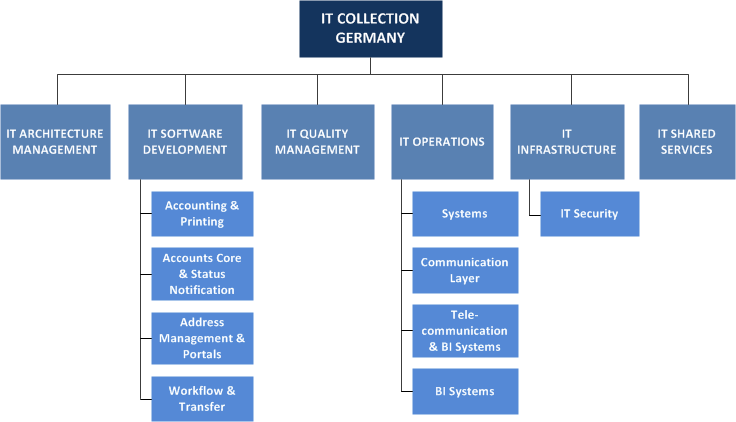
\includegraphics[scale=0.78]{img/IT_Collection_Germany_Organisation.png}
  \caption{Organisationsstruktur IT Collection Germany}
  \caption*{\textbf{Quelle:} eigene Darstellung}
  \label{fig:organisationsstruktur}
\end{figure}
Innerhalb der Abteilungen IT Softwareentwicklung und IT Operations sind die Aufgaben auf mehrere Teams aufgeteilt von denen jedes Team einen abgesteckten Zuständigkeitsbereich verantwortet.

Ein weiterer Bereich ist der Fachbereich. Dort wird ebenso von Abteilungsebene bis runter auf Teamebene gruppiert. Es gibt Teams, die nur Forderungen eines gewissen Mandanten (Auftraggeber) bearbeiten oder Teams wie das Special Research Team (SRT), das sich um die Ermittlung wichtiger Informationen zum Schuldner kümmert. Der Fachbereich hat abhängig von ihrem Aufgabenbereich auch nur auf gewisse Forderungen und Benutzeroberflächen im System Zugriff.

\textbf{Inkassosoftware Cosima}

Die digitale Prozessunterstützung wird von der eigens entwickelten Client-Server-Anwendung Cosima übernommen. Es basiert auf der Programmiersprache Java und wurde deshalb komplett in Java-Swing entworfen. Mittlerweile besteht Cosima aus mehreren einzelnen Services und einer Clientanwendung, die jeder Sachbearbeiter auf seinem Rechner hat. Cosima wurde ursprünglich am Entwicklerstandord Baden-Baden konzipiert und entwickelt. Zu dem Zeitpunkt war auch noch ein weiteres Softwaresystem namens Ikaros im Einsatz. Mit dem Ziel auf eine einheitliche Softwarelösung umzusteigen, wurde sich letzten Endes für die Lösung aus Baden-Baden entschieden. Inzwischen sind die Daten aus dem Ikaros Systems komplett nach Cosima migriert worden und Ikaros wird nicht mehr aktiv eingesetzt.

Die Inkassosoftware findet in den verschiedensten Fachbereichen und Prozessabläufen anwendung. Cosima wird zum einen als Speichermedium für benötigte Mandanteninformationen sowie jeglich rechtlich erlaubte und für den Inkassoprozess benötigte Informationen zu Forderungen und Schuldnern, verwendet. Zum anderen unterstützt die Software die Sachbearbeiter bei ihrer täglichen Arbeit. 

Durch den ständigen Wandel von Gesetzen, Richtlinien und Anforderungen, muss Cosima durchgehend angepasst und erweitert werden. Darunter leidet auch die Qualität. Mit Blick auf die Performance und die damit verbundene Software-Ergonomie werden daher immer wieder IT getriebene Softwareprojekte ins Leben gerufen. bei denen es darum geht die Softwarequalität zu steigern. So kümmert sich besonders das IT Quality Management darum, dass während des Entwicklungsprozesses gewisse Richtlinien und Normen eingehalten werden. Außerdem werden bestehende Benutzeroberflächen, die den Anforderungen nicht mehr gerecht werden, weil sie unübersichtlich oder ineffizient sind, nach und nach renoviert.

%%%%%%%%%%%%%%%%%%%%%%%%%%%%%%%%%%%%%%%%%%%%%%%%%%%%%%%%%%%%%%%%%%%%%%%%%%%%

\subsection{Ist-Situation und Problemstellung}
Durch zusätzliche Features und Anforderungen ist Cosima mit der Zeit immer weiter gewachsen. Meist bestehen solche Features aus einer erweiterten Datenstruktur und letztendlich einer Veränderung, Anpassung beziehungsweise Erweiterung von Benutzerschnittstellen. Cosima besitzt über achthundert verschiedene Dialoge zur Anzeige und Bearbeitung von Daten. Einer dieser Dialoge ist für die Verwaltung von Schuldnerinformationen zuständig. Genauer gesagt werden dort Informationen zur Lebenssituation, Finanzsituation und dem Vermögen eines Schuldners gespeichert. Die Oberfläche wird mittlerweile für mehr als nur einen Anwendungsfall eingesetzt und besitzt daher einige Bedien- und Eingabeelemente, die für den ursprünglichen Use-Case unrelevant sind. Dadurch das der Dialog für mehrere Anwendungsfälle verwendet wird aber nicht jeder Anwendungsfall die kompletten Daten aus dem Dialog benötigt, wird ein Overhead\footnote{Overhead = Daten die nicht zu den primären Nutzdaten zählen} erzeugt, der das Arbeiten mit dem Dialog unnötig verkompliziert. Sachbearbeiter finden den Dialog inzwischen sehr unübersichtlich und die Benutzung eher schwerfällig und ineffizient.

Einer dieser Anwendungsfälle tritt immer dann auf, wenn Schuldner ihre ausstehenden Forderungen nicht begleichen möchten oder nach eigenen Angaben nicht können. In diesen Fällen wird dann eine Zwangsvollstreckung eingeleitet. Dazu wird der Schuldner von einem, durch die \gls{AFS} beauftragten Gerichtsvollzieher, heimgesucht, um einen Vermögensantrag zu seiner aktuellen Lebens- und Finanzsituation auszufüllen. Dieser Antrag besitzt einen standardisierten Aufbau und wird nach dem er vom Schuldner ausgefüllt wurde an die \gls{AFS} geschickt. Als nächstes wird durch das System automatisch ein Listeneintrag\footnote{Listeneintrag = ein Arbeitsauftrag der für Sachbearbeiter im System erscheint} erstellt, der einem zuständigen Sachbearbeiter zugeteilt wird. Im ersten Arbeitsschritt öffnet der Mitarbeiter das, als PDF vorliegende, Dokument auf einem seiner Monitore. Gleichzeitig öffnet er den Dialog für Schuldnerinformationen auf einem weiteren Monitor. Nach und Nach werden dann die vorliegenden Angaben aus dem Vermögensantrag in den Dialog übernommen und am Ende abgespeichert. Als grafische Darstellung des beschriebenen Use-Cases, liegt im Anhang ein Prozessdiagramm (Abb. \ref{fig:zwangsvollstreckungProzess}) vor.

Das Problem speziell in diesem Fall liegt darin, dass der Sachbearbeiter für zwei untereinander folgenden Informationen aus dem Antrag teilweise an mehrere verschiedenen Stellen in dem Dialog springen muss, um diese zu übernehmen. Der Arbeitsablauf wird durch solche Sprünge unterbrochen und der Bearbeiter muss sich häufig neu orientieren. Zudem ist der Dialog mit zunehmender Anzahl an Bedienelementen, auch immer unübersichtlicher geworden. Sachbearbeiter berichten immer wieder von einer zu komplexen und ineffizienten Benutzeroberfläche. Grundsätzlich brauchen auch neue Arbeitskräfte bei der Einarbeitung mit diesem Dialog länger als gewünscht. Aus diesen Gründen sind sich die Beteiligten einig das eine Veränderung durchgeführt werden muss. Der aktuelle Dialog ist in die Jahre gekommen und entspricht nicht mehr den Anforderungen der Verantwortlichen.

%%%%%%%%%%%%%%%%%%%%%%%%%%%%%%%%%%%%%%%%%%%%%%%%%%%%%%%%%%%%%%%%%%%%%%%%%%%%

\subsection{Zielsetzung, Forschungsfrage und Hypothesen}
Die Ist-Situation inklusive ihrer Problemstellung, dient als Ansatzpunkt für mein Projektziel, das sich in zwei Unterziele aufteilt. Der erste Teil des Ziels besteht aus der Konzeption und Implementierung eines neuen Dialogs für die Eingabe von Vermögensverzeichnissen. Im zweiten Schritt soll dieser Dialog mit dem bestehenden Dialog für Vermögensverzeichnisse auf Basis einer empirischen Datenerhebung in den Disziplinen Ergonomie, Effizienz und Performance verglichen werden. Die zu erhebenden Daten bestehen ebenfalls aus zwei Teilen. Zum einen den objektiv technisch erhobenen Daten und zum anderen den mehr subjektiv und aus einem Fragebogen entstammenden Daten. Am Ende soll ein neuer Dialog zur Verfügung stehen, der dem Sachbearbeiter eine ergonomische, anwendungsfallorientierte und performante Eingabe von Vermögensverzeichnissen ermöglicht. Dabei soll dieses Projekt der erste Schritt für die Ablösung des alten Dialoges dienen. 

Im Verlaufe der Abschlussarbeit gilt es das zu erreichende Ziel auch hinsichtlich aufgestellter Hypothesen und Antithesen zu überprüfen. Neben den Thesen gibt es eine zentrale Forschungsfrage, die mit den gewonnen Erkenntnissen und Ergebnissen am Ende der Thesis beantwortet werden soll. Die Hauptfrage mit der sich beschäftigt werden soll lautet: \glqq Ist der neue Dialog für Vermögensverzeichnisse ergonomischer und effizienter als der bisherige Dialog?\grqq{}.

Zusätzlich zu der Forschungsfrage werden Hypothesen aufgestellt, die im Ergebnisteil überprüft werden sollen. Die Hypothesen dienen später als Hilfe bei der Beantwortung der Forschungsfrage. Eine der zu verifizierenden Hypothesen in diesem Kontext heißt: \glqq Wenn der neue Dialog verwendet wird, dann sinkt die durchschnittliche Bearbeitungszeit bei der Anlage von Vermögensverzeichnissen\grqq{}. Eine weitere damit verbundene Hypothese lautet: \glqq Je weniger Bedienelemente die Oberfläche besitzt desto weniger Interaktionen finden durch den Sachbearbeiter statt\grqq{}. Im Bereich der Ergonomie wird die Hypothese: \glqq Der neue Dialog wird im Gegensatz zum alten Dialog als ergonomischer empfunden\grqq{} aufgestellt. Zudem werden diese Hypothesen ebenfalls als zu untersuchenden Antithesen umformuliert: \glqq Wenn der neue Dialog verwendet wird, dann stagniert oder steigt die durchschnittliche Bearbeitungszeit bei der Anlage von Vermögensverzeichnissen\grqq{}, \glqq Je mehr Bedienelemente eine Oberfläche besitzt, desto weniger Interaktionen finden durch den Sachbearbeiter statt\grqq{} und \glqq Der neue Dialog wird im Gegensatz zum alten Dialog als nicht ergonomischer empfunden\grqq{}.

%%%%%%%%%%%%%%%%%%%%%%%%%%%%%%%%%%%%%%%%%%%%%%%%%%%%%%%%%%%%%%%%%%%%%%%%%%%%

\subsection{Aufbau und Vorgehen}
Die Ausarbeitung gliedert sich in sieben Kapitel. Die ersten beiden Kapitel \textit{Vorwort} und \textit{Abstract} schaffen keinen inhaltlichen Mehrwert, sondern dienen der Motivation und als Zusammenfassung der Inhalte und Ergebnisse dieser Bachelorarbeit.

Das Kapitel \textit{Einleitung} führt grundsätzlich in das Thema ein. Dazu wurde die Ist-Situation und das bestehende Problem beschrieben. Darauf folgen dann \textit{Zielsetzung, Forschungsfrage und Hypothesen}, die es am Ende der Arbeit zu beantworten und zu überprüfen gilt. In dem letzten Teil der Einleitung wird das Partnerunternehmen Bertelsmann SE \& Co. KGaA und die Tochtergesellschaft \gls{AFS} mit ihrem Inkassounternehmen \gls{IFM} vorgestellt.

Im darauf folgenden Kapitel geht es darum, die benötigten theoretischen \textit{Grundlagen} zu erklären. Dafür wird auf die \textit{eingesetzten Technologien} und Werkzeuge, die im Projektgeschehen benutzt wurden, eingegangen. Im Anschluss folgt der thematische Einstieg in die \textit{Software-Ergonomie} zu der einige Begriffe definiert und \textit{Gestaltgesetze, Normen, Richtlinien, Verordnungen} sowie \textit{Heuristiken} zum Designen von Benutzeroberflächen vorgestellt werden. Im Kapitel \textit{Evaluation von Software-Ergonomie} werden zuerst verschiedene Zieldefinitionen und die zwei \textit{Arten der Evaluation} vorgestellt. Im Anschluss werden dann, die für das Projekt relevanten, \textit{Erhebungsmethoden} erläutert. Zu diesen werden einzelne Vor- und Nachteile sowie \textit{Gütekriterien}, anhand derer die Qualität der Erhebung gemessen wird, genauer beleuchtet. Im darauf folgenden Teil wird der Ansatz des \textit{Usability-Engineerings} erläutert. In dem Zusammenhang wird ein Vorgehensmodell vorgestellt und der Begriff Nutzungskontext genauer betrachtet. Als nächstes wird im Abschnitt \textit{statistische Datenanalyse} der Grundstein für die Auswertungen im Kapitel Ergebnisse und Diskussion gelegt. Es werden sowohl Grundbegriffe der Statistik erklärt, als auch mehrere Verfahren zur Auswertung und Aufbereitung von Daten gezeigt. Im letzten Teil der Grundlagen wird die \textit{\gls{KNA}} vorgestellt. Diese soll als zusätzliches Kriterium in der Evaluation dienen.

In Kapitel fünf \textit{Entwicklung der neuen Benutzeroberfläche für Vermögensauskünfte} geht es darum die neue Benutzerschnittstelle für Vermögensauskünfte, mit Hilfe der Empfehlungen und Vorgaben aus Kapitel 4.2, zu konzipieren und für einen produktiven Test zu implementieren. Dabei wird das \textit{Vorgehensmodell für den Entwicklungsprozess}, das in Kapitel 4.4.1 vorgestellt wurde, auf den Projektkontext angewandt. Es werden 

In dem Kapitel \textit{Evaluation} wird das Ziel und der Aufbau der Evaluation festgelegt. Für die anschließende Durchführung der \textit{empirische Datenerhebung} werden zunächst die eingesetzten \textit{Erhebungsmethoden} und \textit{Messinstrumente} bestimmt. Als zusätzliches Kriterium für die Evaluation wird eine Kosten-Nutzen-Analyse durchgeführt.

Im Anschluss an die empirische Erhebung werden Ergebnisse präsentiert, interpretiert und diskutiert. Dazu werden zunächst die erhobenen Daten, bezogen auf ihre Erhebungsmethode bzw. Analysemethode, ausgewertet und anschließend in einer Zusammenfassung auf gegenseitige Einflüsse und Wirkungen untersucht. Schlussendlich werden in der Zusammenfassung die Ziele, Hypothesen und die Forschungsfrage erneut aufgegriffen und beantwortet bzw. überprüft.

Im abschließenden Kapitel wird mit Hilfe der erzielten Ergebnisse ein \textit{Ausblick} in nachfolgende Projekte und Handlungsalternativen gegeben.



